%! TEX root = ./maimain.tex

\lecture{10}{Week 5}{Basic x86 Architecture and C Control Flow}

\subsubsection{x86 Integer Arithmetic}

\paragraph{Some Arithmetic Operations}
Important two-operand instructions:

\begin{tabular}{l l}
    \code{addl} & $Dest = Dest + Src$\\
    \code{subl} & $Dest = Dest - Src$\\
    \code{imull} & $Dest = Dest * Src$\\
    \code{sall} & $Dest = Dest << Src$\\
    \code{sarl} & $Dest = Dest >> Src$\\
    \code{shrl} & $Dest = Dest >> Src$\\
    \code{xorl} & $Dest = Dest\ \hat{}\ Src$\\
    \code{andl} & $Dest = Dest \& Src$\\
    \code{orl} & $Dest = Dest | Src$
\end{tabular}

There is no difference between arithmetic and logic shift left, and hence, the instructions \code{sall} and \code{shll} are equivalent.

Two-operand instructions store the result of the calculation in one of the operands. There is not separate register. This is a limitation which stems from the early days where registers were rar but nowadays, where registers are actually stored in a register file with +200 resists which is is no longer an issue. (The name of a regster is just a temporary reference to an entry of the register file)

All operations act on the binary numbers and there is no notion of signed or unsigned integers. That is because it does not make any difference for the computation!

Important one operand instructions:

\begin{tabular}{l l}
    \code{incl} & $Dest = Dest + 1$\\
    \code{decl} & $Dest = Dest - 1$\\
    \code{negl} & $Dest = -Dest$\\
    \code{notl} & $Dest = \tilde{} Dest$
\end{tabular}

\paragraph{\code{lea} for Arithmetic Expressions}
The compiler clever and makes us of \code{lea} for arithmetic instructions. This is especially powerful when replacing a multiplication by \code{lea} and shifts.

The C compiler is better in assembly than we humans :)

There is again a version for different sized: \code{leal} etc.

\subsubsection{Condition Codes}
Condition codes are extra bits, like one-bit registers. But they are packed into the status register. They provide us extra information about executed operations.

They have names and they are set (implicitly) during arithmetic instructions (but \textbf{not} by \code{lea}):
\begin{description}
    \item[CF:] Carry Flag (for unsigned)
        \begin{itemize}
            \item Set if carry out of most significant bit
            \item i.e unsigned overflow
        \end{itemize}
    \item[ZF:] Zero Flag
        \begin{itemize}
            \item Set if result is equal to $0$
        \end{itemize}
    \item[SF:] Sign Flag (for signed)
        \begin{itemize}
            \item Set equal the most significant bit
            \item i.e. if interpreted as signed, the result is negative
        \end{itemize}
    \item[OF:] Overflow Flag (for signed)
        \begin{itemize}
            \item Set to \code{( a > 0 \&\& b > 0 \&\& t < 0) || (a < 0 \&\& b < 0 \&\& t >= 0)}
            \item i.e. if interpreted as signed, the results overflows
        \end{itemize}
\end{description}

Condition codes can also be set explicitly using the \code{cmpl/cmpq Src2, Src1} instruction. This instruction computes i.e. \code{Src1 - Src2} and sets the conditional flags (but does not store the result of the computation).

The second instruction to set the condition codes explicitly is \code{testl/testq Src2, Src1}. It computes \code{Src1 \& Src2}, sets the condition codes but again, not the result. This instruction is very useful when one instruction is a mask.

\paragraph{Read Condition Codes}
The \code{SetX Dest} instruction computes an expression based on the current flags and writes that to the low-byte of a register. There are the following flavours:

\begin{tabular}{l l l}
    \code{sete}  & $ZF$                                     & Equal/Zero\\
    \code{setne} & $\tilde{} ZF$                            & Not Equal/Not Zero\\
    \code{sets}  & $SF$                                     & Negative\\
    \code{setns} & $\tilde{} SF$                            & Non-Negative\\
    \code{setg}   & $\tilde{} (SF\ \hat{}\ OF) \&\ \tilde{} ZF$ & Greater (Signed)\\
    \code{setge}   & $\tilde{} (SF\ \hat{}\ OF)$                & Greater or Equal (Signed)\\
    \code{setl}   & $(SF\ \hat{}\ OF)$                         & Less (Signed)\\
    \code{setle}   & $(SF\ \hat{}\ OF) | ZF$                    & Less or Equal (Signed)\\
    \code{seta}   & $\tilde{} CF \&\ \tilde{} ZF$             & Above (Unsigned)\\
    \code{setb}   & $CF$                                     & Below (Unsigned)\\
\end{tabular}

$32$ bit instructions set the higher-order bit, of e.g. \code{\%rax} to the same value when writing to \code{\%eax}. The \code{setX} operations are not $32$ bit instructions and therefore do not modify the higher-order bytes but only sets the least significant byte! \code{xor} is a cheap way to set a register to $0$. So with the combination of \code{xor} and \code{setX} we can move a certain flag wo any register we want.

\code{movzbl} moves a byte to a longword and fills with leading zeros. \code{movsbl} is equivalent, but in contrast to \code{movzbl}, it sign-extends the value. Using one of these instructions, we do not have to explicitly zero the register.

\paragraph{Jumping}
The \code{jX Tag} instructions jump depending on some conditional codes. There are the following flavours:

\begin{tabular}{l l l}
    \code{jmp} & $1$ & Unconditional\\
    \code{je}  & $ZF$                                     & Equal/Zero\\
    \code{jne} & $\tilde{} ZF$                            & Not Equal/Not Zero\\
    \code{js}  & $SF$                                     & Negative\\
    \code{jns} & $\tilde{} SF$                            & Non-Negative\\
    \code{jg}   & $\tilde{} (SF\ \hat{}\ OF) \&\ \tilde{} ZF$ & Greater (Signed)\\
    \code{jge}   & $\tilde{} (SF\ \hat{}\ OF)$                & Greater or Equal (Signed)\\
    \code{jl}   & $(SF\ \hat{}\ OF)$                         & Less (Signed)\\
    \code{jle}   & $(SF\ \hat{}\ OF) | ZF$                    & Less or Equal (Signed)\\
    \code{ja}   & $\tilde{} CF \&\ \tilde{} ZF$             & Above (Unsigned)\\
    \code{jb}   & $CF$                                     & Below (Unsigned)\\
\end{tabular}

There is also conditional move \code{cmovX src, dest} which moved from source to destination depending on the condition. But is is not that useful. Not even RISC had this feature.
This is most of the x86 assembly we will cover.

\subsection*{C Control Flow}
\subsubsection{If-then-else}
\code{If then else} statements can be compiled as conditional branches. In fact, any conditional can we rewritten as a conditional with if clause only (no else) with a goto in its clause. One should not write code like that, but let the compiler to that work.

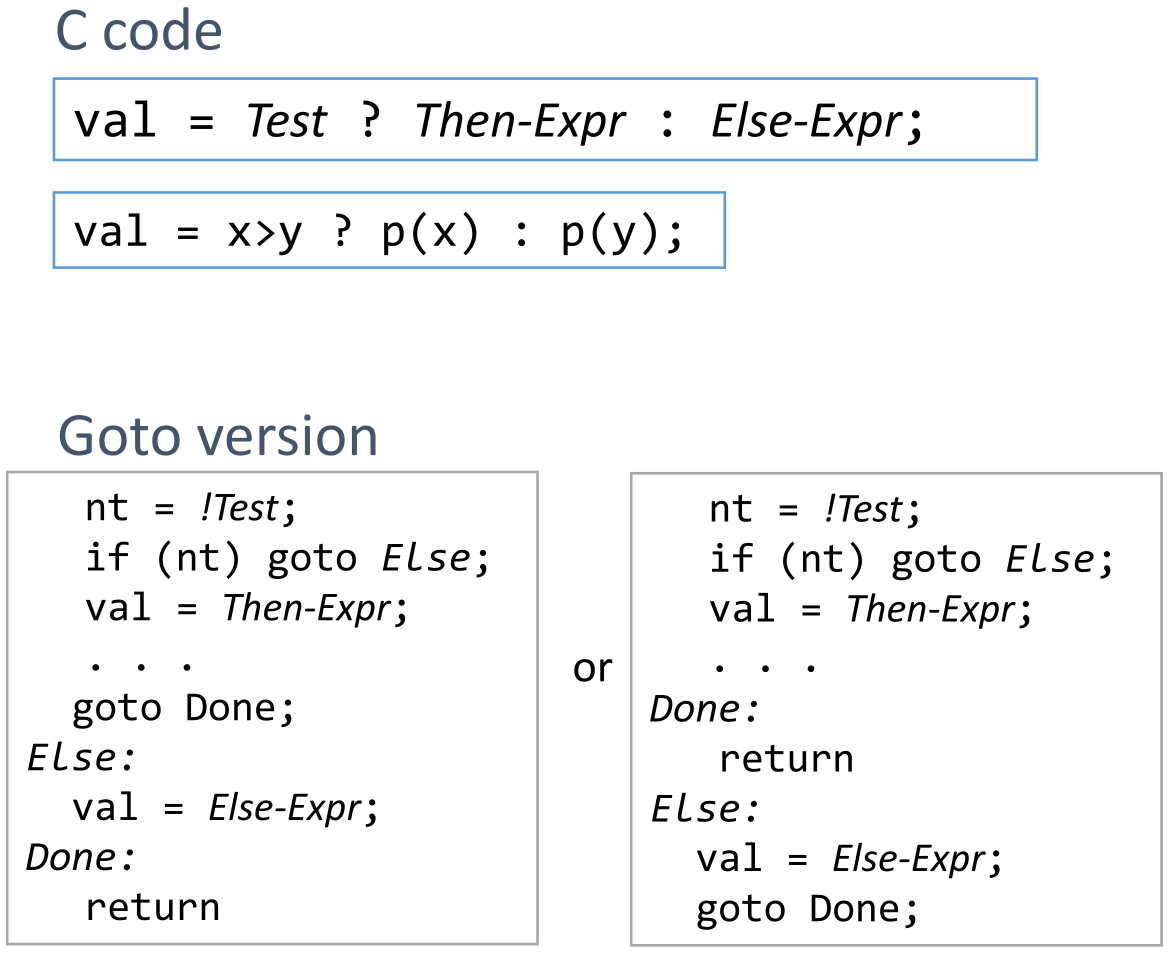
\includegraphics[width=0.5\textwidth]{10_conditional_goto.png}

Both orderings are very similar. It depends on the hardware which one is better.

Sometimes the compiler uses conditional move \code{cmovX src, dest} instead of jumps. Generally, this is more efficient event though we may have to do more work since all instructions get executed. But if the additionally work dominates or if the execution of both branches have side effects, one should not use conditional moves.

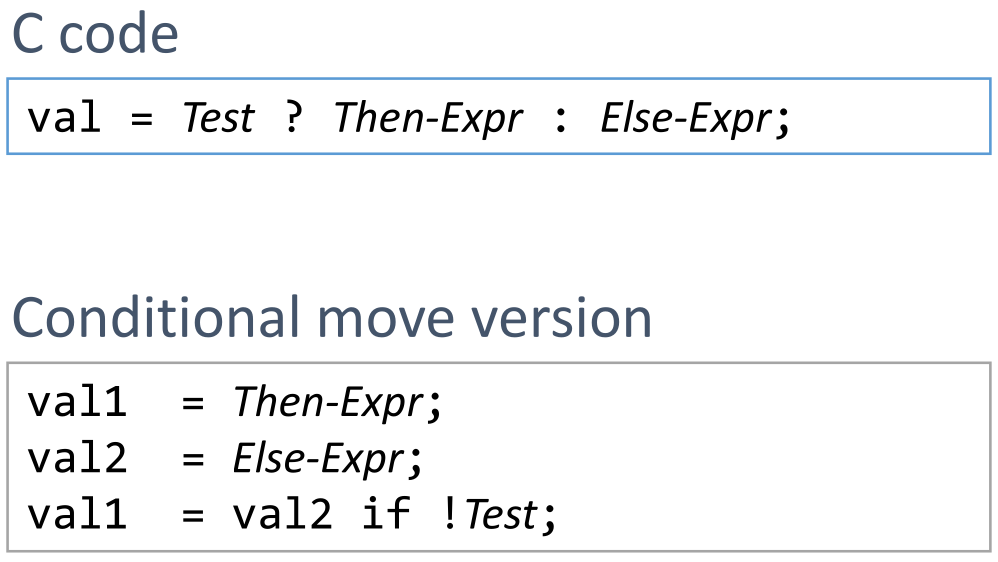
\includegraphics[width=0.5\textwidth]{10_conditional_mov.png}

\subsubsection{\code{do-while} loops}
\code{do while} are fancy conditionals with a jump. A conditional backward branch is used to continue looping as long as the condition is true.

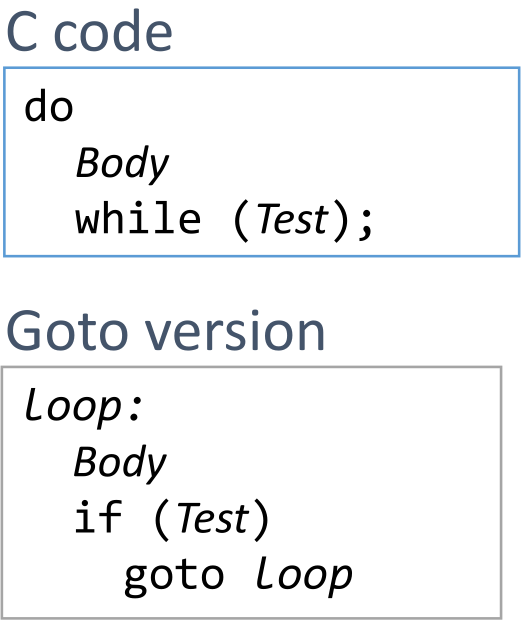
\includegraphics[width=0.5\textwidth]{10_dowhile.png}

\subsubsection{\code{while} loops}
GCC used to convert \code{while} to \code{do-whiles} with an additional conditional jump at the beginning. However, nowadays, there are separate blocks for the conditional check and the loop. At the beginning we jump to the conditional, called middle, and jump to the loop, if the condition is meat. This method is called \code{jump to middle}.

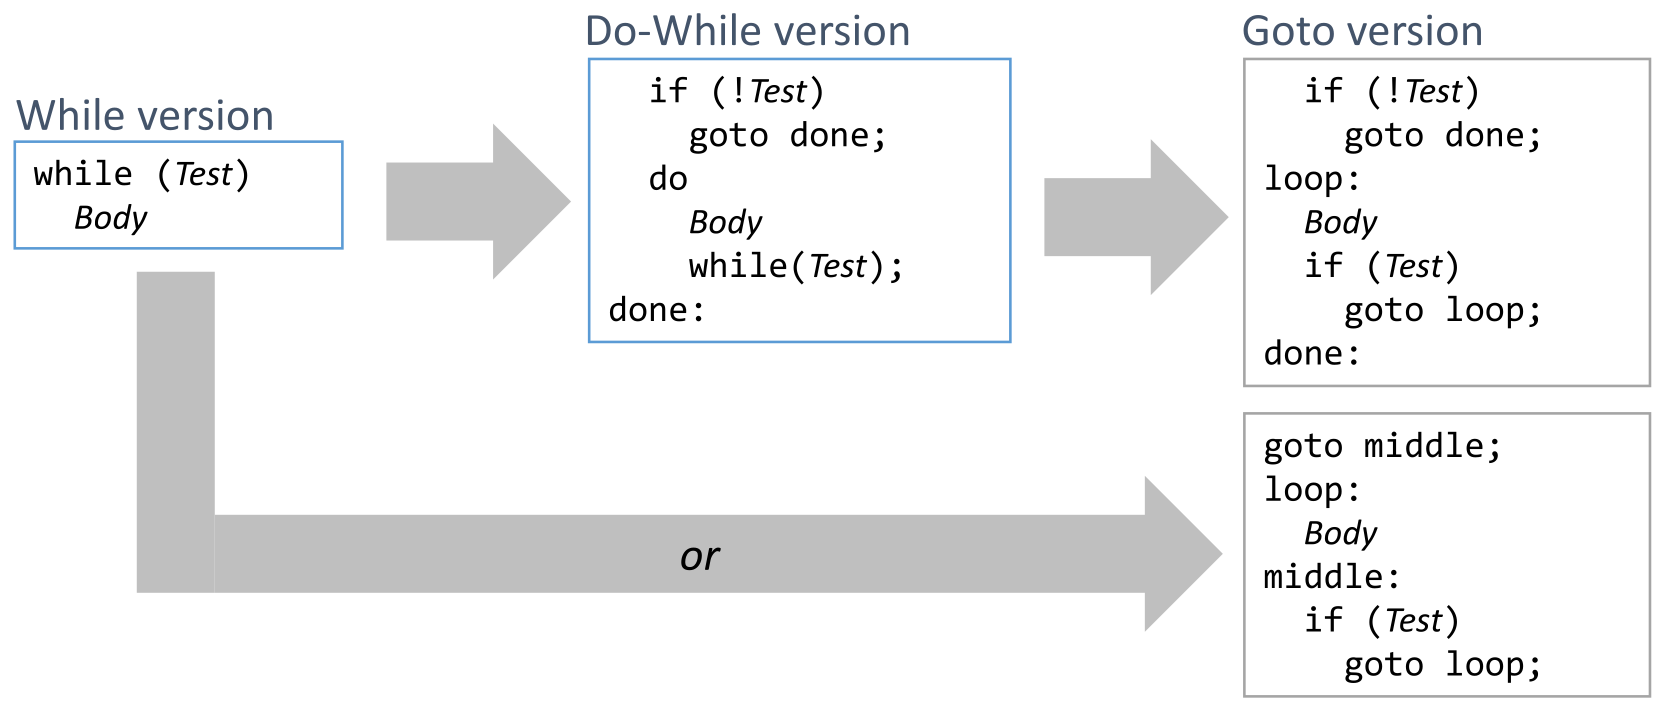
\includegraphics[width=0.8\textwidth]{10_while.png}

\subsubsection{\code{for} loops}
Are \code{while} loops with an initialisation.

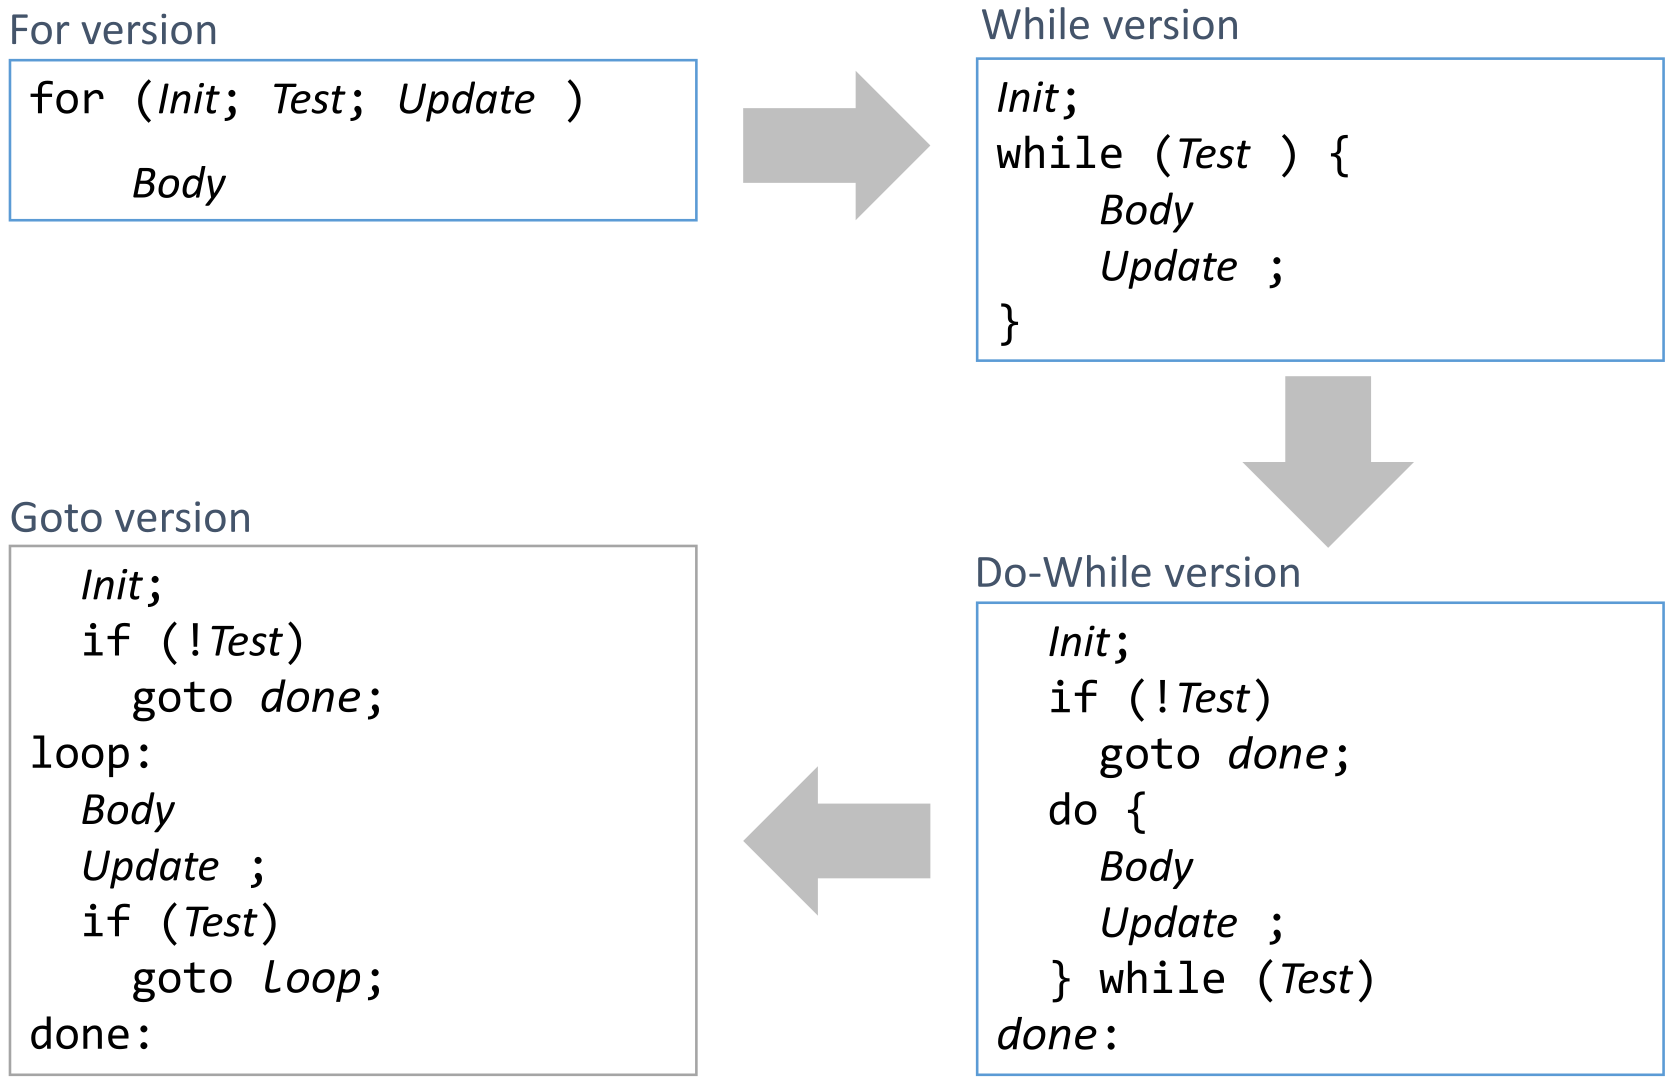
\includegraphics[width=0.8\textwidth]{10_for.png}

\subsubsection{\code{switch} statements}
The obvious way is \code{if then else}, but nobody does it. There are two kinds of statements, one where the values are compact, and switch when the values are not compact.

\subsubsection{Additional Statements:}
Anything starting with a dot in assembler is stuff not in the machine code. This is related to linking and information about what is in this file. This is handy for debugging.

\code{.text} says that code is following

\code{.global} means that the scope of the following name is global.

\code{.type} tells the type of a variable/function.
